
\section{Simulation}\label{sec:simulation}
% Simulation:
%%  Mean control results   (image and plot(s) )
%%  Variance Control      (image and plot(s) )
%%  Hybrid control   (image and plot(s) )

\subsection{Controlling the mean position}

For controlling mean position, we use a PD controller. Our control input is the force we make, goal positions are the desired positions, and we have our mean position and mean velocity. So we have:
\begin{align}
u_x &= K_{p}(x_{goal} - \bar{x}) + K_{d}(0-\bar{v}_x) \nonumber\\
u_y &= K_{p}(y_{goal}  - \bar{y}) + K_{d}(0-\bar{v}_y)  \label{eq:PDcontrolPosition}
\end{align}
where $K_{p}$ is the proportional gain, and $K_{d}$ the derivative gain. We performed a parameter sweep to identify the best values.  Representative experiments are shown in Fig.~\ref{}. 100 robots were used and the maximum speed was 3 meter per second. With these parameters, we showed that the best values are  $K_{p}= 4$, and  $K_{d} = 1$~\ref{fig:gainValues}.



%give PID control law, explain experiment (number of robots, maximum speed, ).

%contrast controllers -- as is typical with PID control laws, we can tune the response to meet desired specifications.


%image showing varying P control  %I want  1.5 cycles, nicely cropped,  all starting at same time

%image showing varying D control

%image showing varying the number of robots n % is this needed?

%\subfloat[][Vary Visual Feedback]{\label{fig:VaryVis}
%\begin{overpic}[width =\figwid]{VaryVisFS.pdf}\end{overpic}}


%\begin{figure}
%        \centering
%        \begin{subfigure}[b]{0.3\textwidth}
%                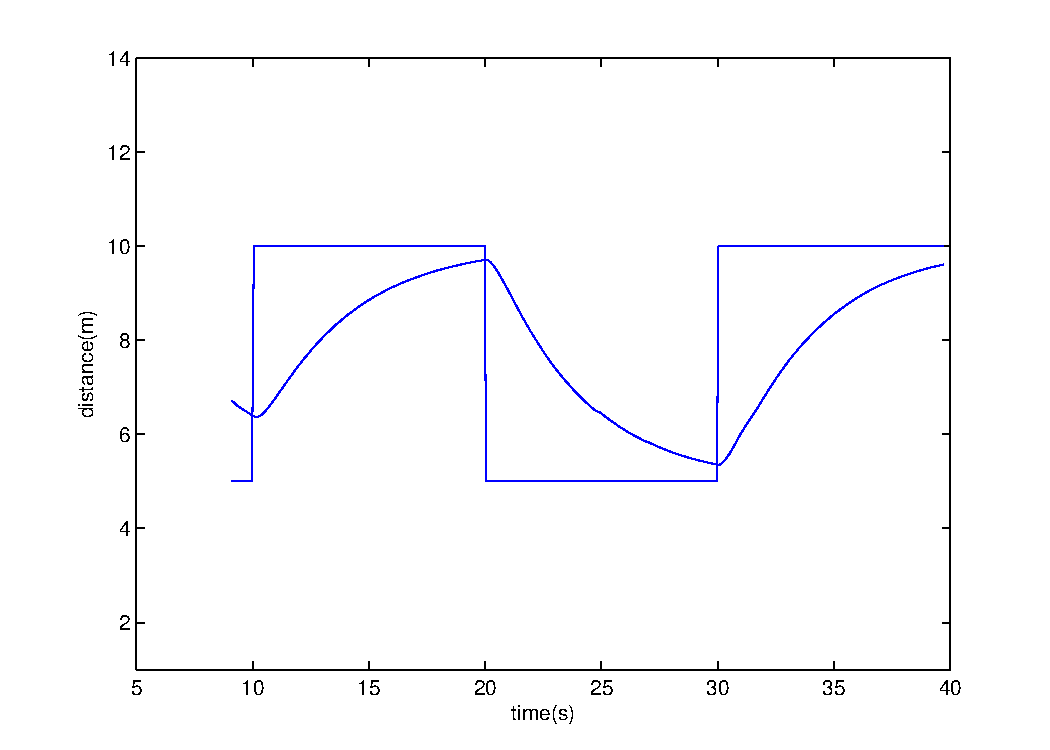
\includegraphics[width=\textwidth]{fig/gain1d1.pdf}
%                \caption{g 1, d 1}
%                \label{fig:gull}
%        \end{subfigure}%
%        ~ %add desired spacing between images, e. g. ~, \quad, \qquad, \hfill etc.
%          %(or a blank line to force the subfigure onto a new line)
%        \begin{subfigure}[b]{0.3\textwidth}
%                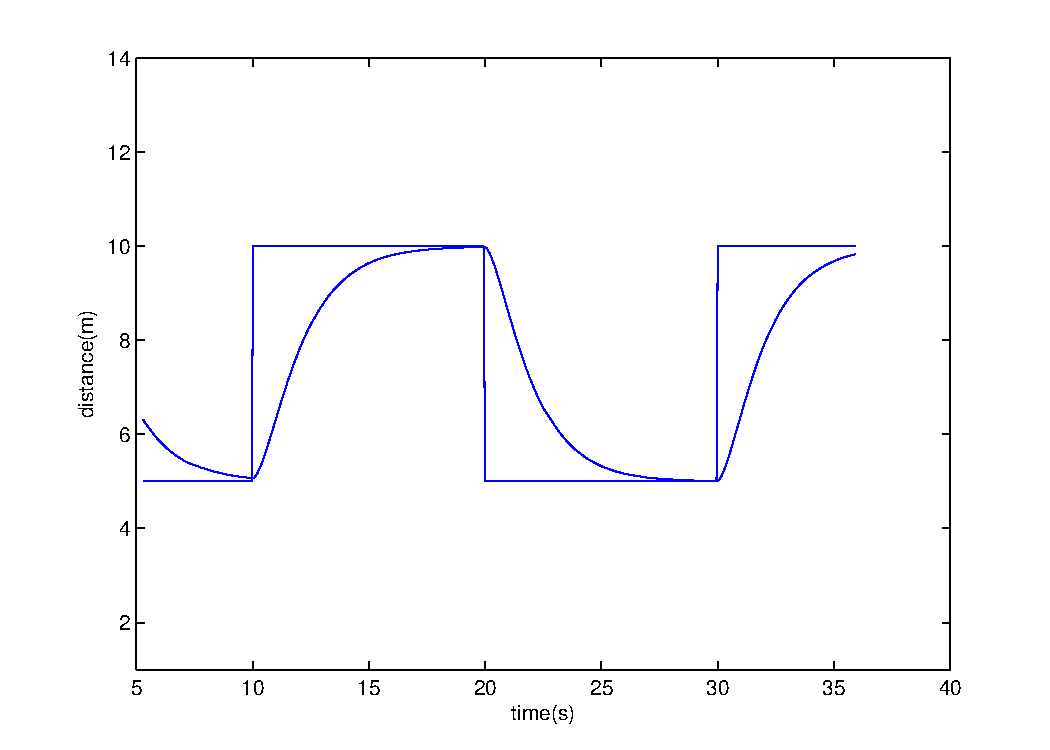
\includegraphics[width=\textwidth]{fig/gain2d1.pdf}
%                \caption{g 2, d 1}
%                \label{fig:tiger}
%        \end{subfigure}
%        ~ %add desired spacing between images, e. g. ~, \quad, \qquad, \hfill etc.
%          %(or a blank line to force the subfigure onto a new line)
%        \begin{subfigure}[b]{0.3\textwidth}
%                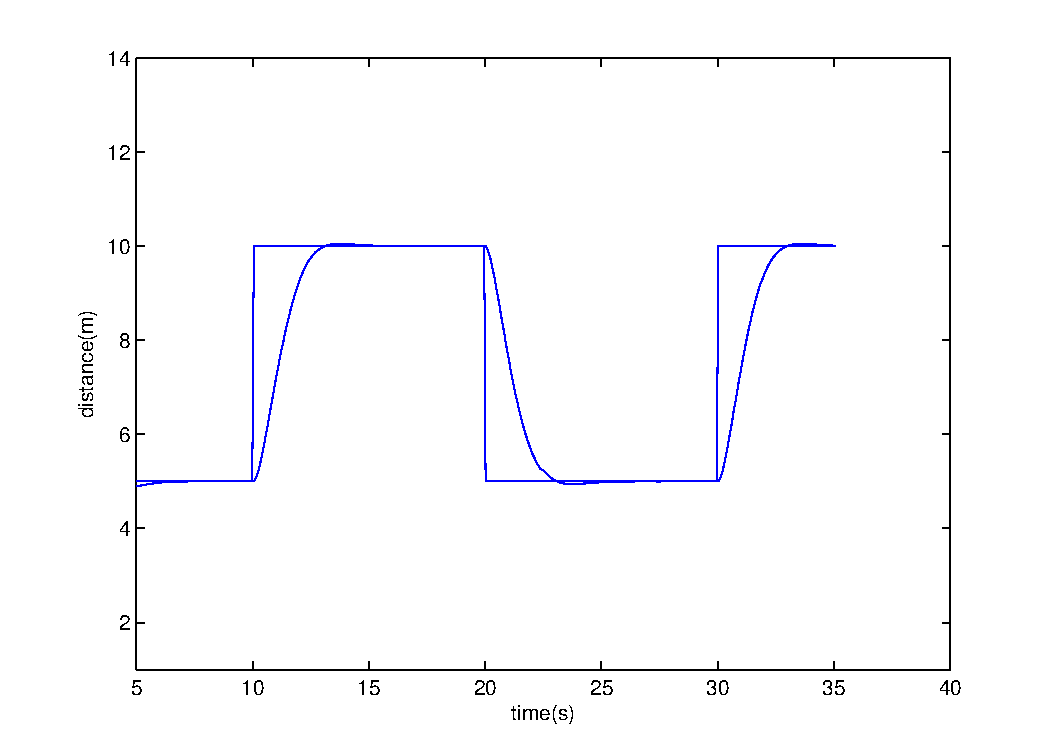
\includegraphics[width=\textwidth]{fig/gain4d1.pdf}
%                \caption{g 4, d 1}
%                \label{fig:mouse}
%        \end{subfigure}
%                \begin{subfigure}[b]{0.3\textwidth}
%                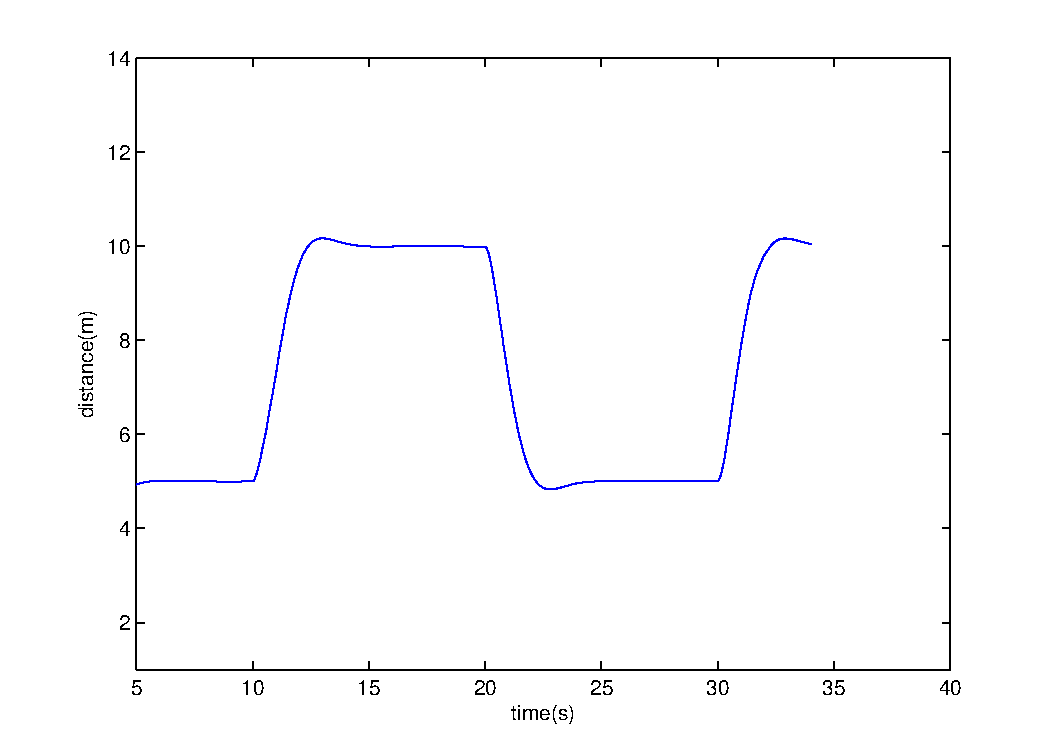
\includegraphics[width=\textwidth]{fig/gain5d1.pdf}
%                \caption{g 5, d 1}
%                \label{fig:gull}
%        \end{subfigure}%
%        ~ %add desired spacing between images, e. g. ~, \quad, \qquad, \hfill etc.
%          %(or a blank line to force the subfigure onto a new line)
%        \begin{subfigure}[b]{0.3\textwidth}
%                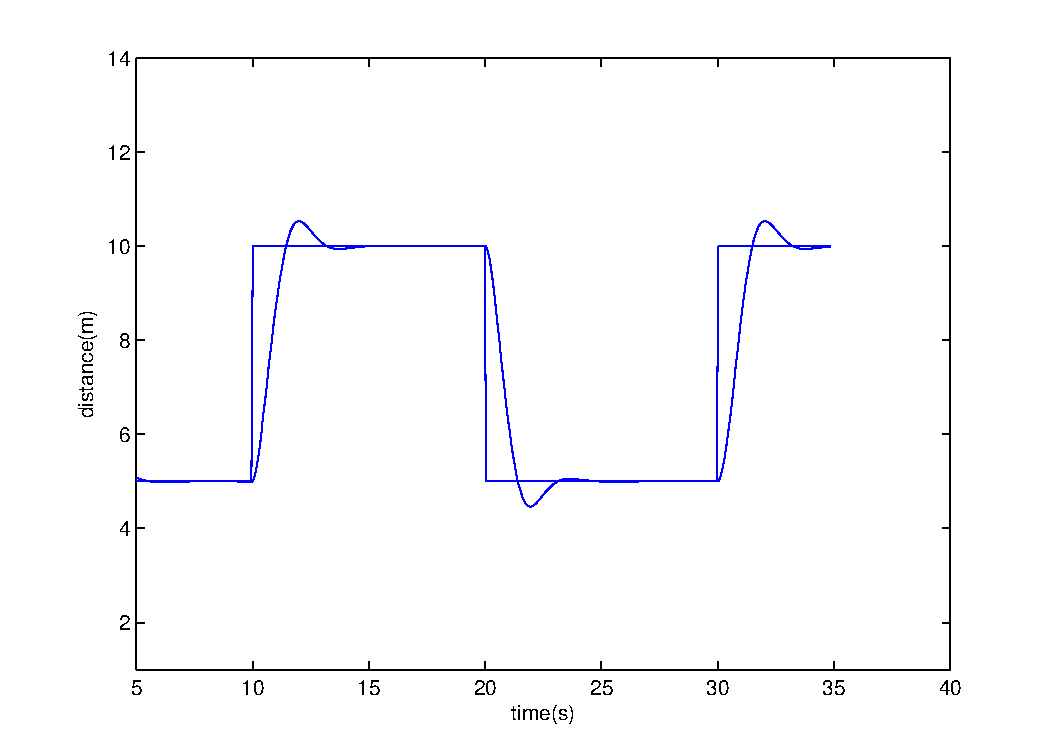
\includegraphics[width=\textwidth]{fig/gain8d1.pdf}
%                \caption{g 8, d 1}
%                \label{fig:tiger}
%        \end{subfigure}
%        ~ %add desired spacing between images, e. g. ~, \quad, \qquad, \hfill etc.
%          %(or a blank line to force the subfigure onto a new line)
%        \begin{subfigure}[b]{0.3\textwidth}
%                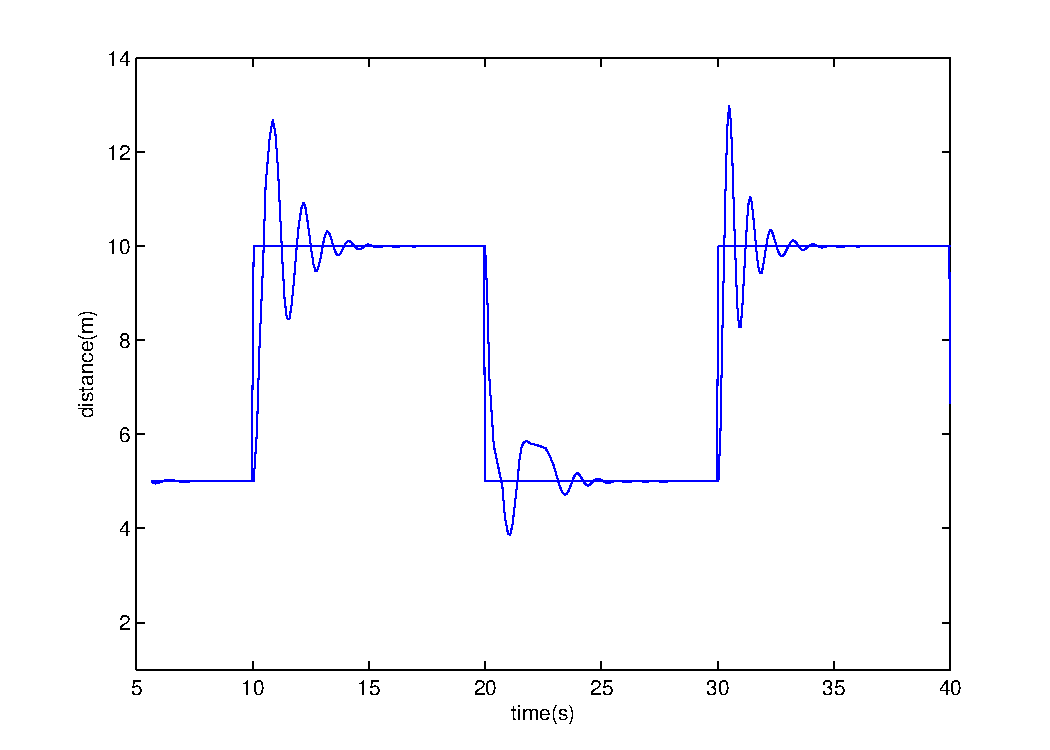
\includegraphics[width=\textwidth]{fig/gain100d1.pdf}
%                \caption{g 100, d 1}
%                \label{fig:mouse}
%        \end{subfigure}
%        \caption{Different Gain Values}\label{fig:gainvalues}
%\end{figure}
%\begin{figure}
%        \centering
%        \begin{subfigure}[b]{0.3\textwidth}
%                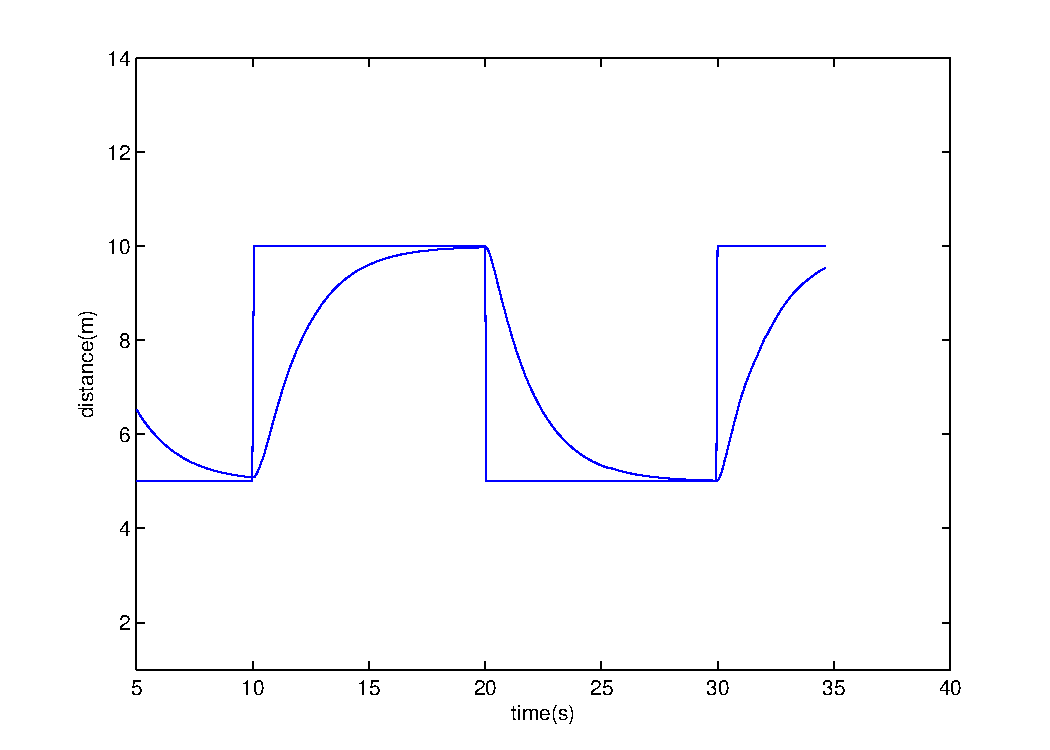
\includegraphics[width=\textwidth]{fig/gain4d2.pdf}
%                \caption{g 4, d 2}
%                \label{fig:gull}
%        \end{subfigure}%
%        ~ %add desired spacing between images, e. g. ~, \quad, \qquad, \hfill etc.
%          %(or a blank line to force the subfigure onto a new line)
%        \begin{subfigure}[b]{0.3\textwidth}
%                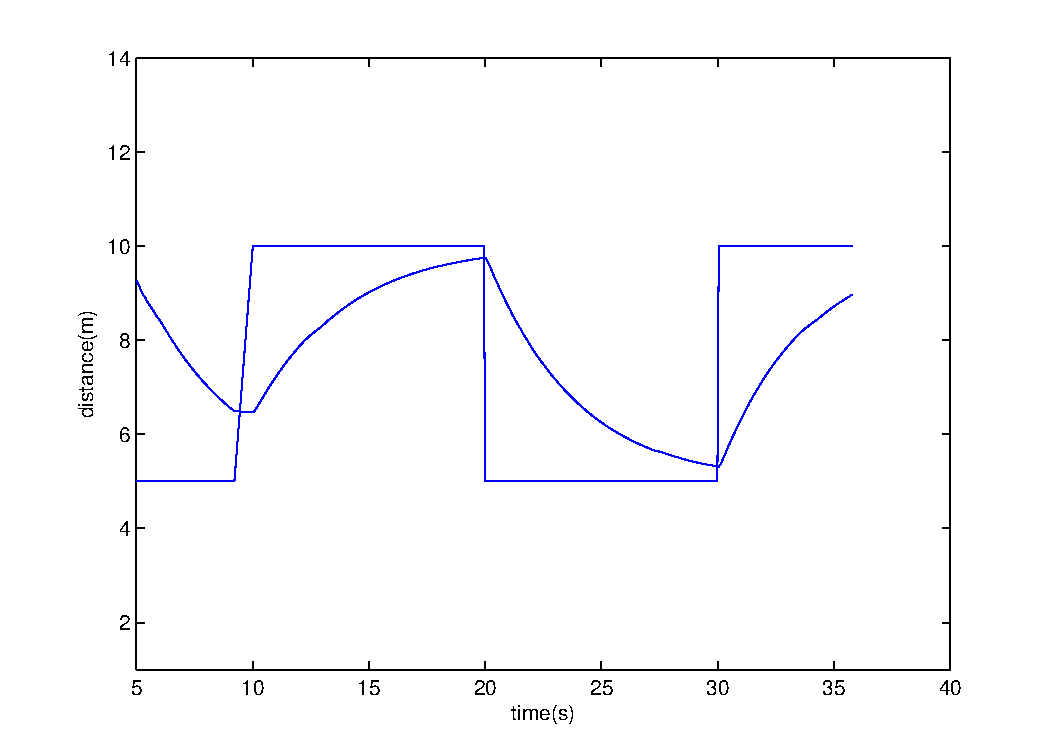
\includegraphics[width=\textwidth]{fig/gain4d4.pdf}
%                \caption{g 4, d 4}
%                \label{fig:tiger}
%        \end{subfigure}
%        ~ %add desired spacing between images, e. g. ~, \quad, \qquad, \hfill etc.
%          %(or a blank line to force the subfigure onto a new line)
%        \begin{subfigure}[b]{0.3\textwidth}
%                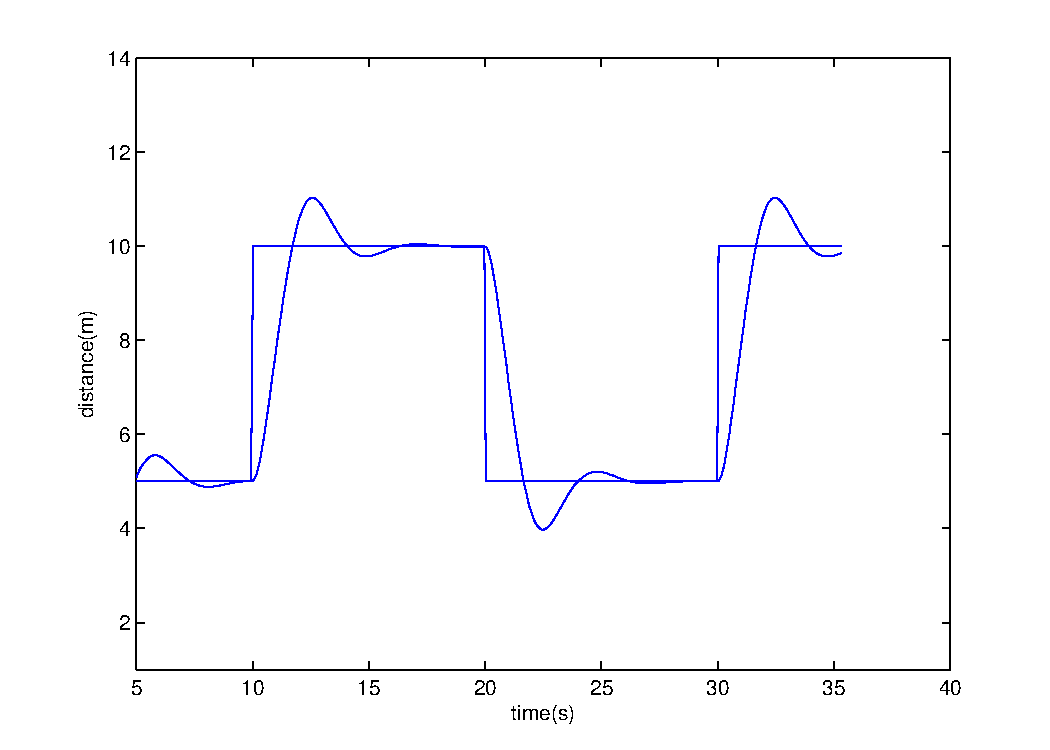
\includegraphics[width=\textwidth]{fig/gain4d05.pdf}
%                \caption{g 4, d 0.5}
%                \label{fig:mouse}
%        \end{subfigure}
%         \caption{Different Derivative Values}\label{fig:animals}
%\end{figure}


\subsection{Controlling the variance}

%cite the control law, explain experiment (number of robots, maximum speed, ).

For variance control we use a hysteresis-based controller discussed in Section~\ref{sec:VarianceControl}.  Waiting is sufficient to increase variance because Brownian noise naturally disperses the swarm.  If faster dispersion is needed, the swarm can be pushed through obstacles such as a diffraction grating or Pachinko board~\cite{Becker2013b}. To decrease the variance, we push the swarm into corners to decrease the variance.  Our algorithm identifies the nearest corner by \todo{ how does it work?}

%\begin{figure}[!htb]
%\captionsetup{justification=centering}
%\minipage{0.32\textwidth}
%  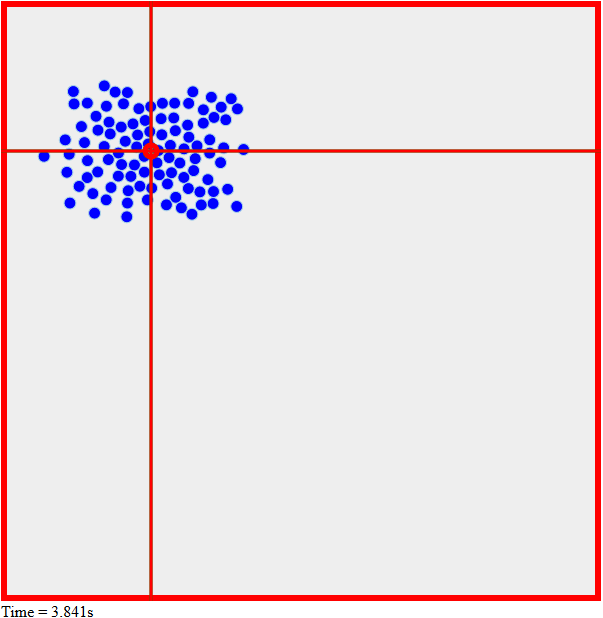
\includegraphics[width=\linewidth]{fig/2DControl3.png}
%  \caption{The goal position is 5 and 5}
%\endminipage\hfill
%\minipage{0.32\textwidth}
%  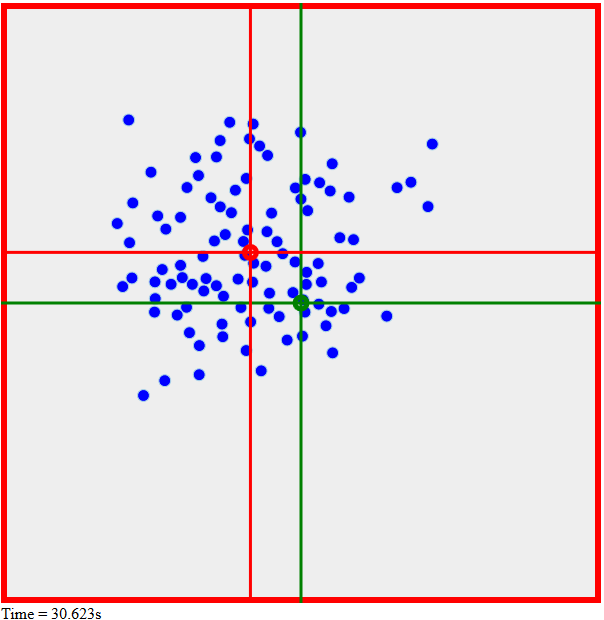
\includegraphics[width=\linewidth]{fig/2DControl2.png}
%  \caption{Going to the goal position}
%\endminipage\hfill
%\minipage{0.32\textwidth}%
%  %\includegraphics[width=\linewidth]{shiva444.eps}
%  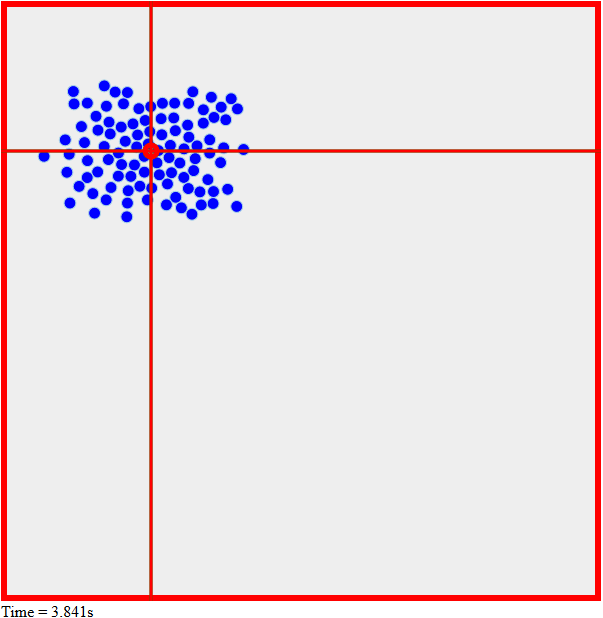
\includegraphics[width=\linewidth]{fig/2DControl3.png}
%  \caption{The goal position is 10 and 10}
%\endminipage
%\end{figure}
%\end{itemize}

contrast controllers -- as is typical with PID control laws, we can tune the response to meet desired specifications.

\todo{image showing varying Brownian noise}

\todo{image showing control x variance and y-variance out of phase}


\subsection{Hysteresis Control of mean and variance}

%\todo{plot showing 1.5 cycles of mean position, and a variance goal.  We might need a longer time}
\begin{figure}
\centering
\begin{overpic}[scale=0.35]{MeanVariance.eps}
\end{overpic}
\vspace{-2em}
\caption{\label{fig:hybrid} Here we control both variance and mean position.
%\vspace{-2em}
}
\end{figure}






